\documentclass{article}
\addtolength{\oddsidemargin}{-.875in}
\addtolength{\evensidemargin}{-.875in}
\addtolength{\textwidth}{1.0in}
\addtolength{\topmargin}{-0.5in}
\addtolength{\textheight}{1.00in}
\usepackage{wrapfig}
\usepackage{sidecap}
\usepackage{hyperref}
\usepackage[pdftex]{graphicx}
\usepackage[utf8]{inputenc}
\usepackage[spanish]{babel}

\title{Reporte de Actividades - Enero 2015 - Febrero 2018}
\author{Jaime E. Forero Romero\\Profesor Asociado - Departamento de
  F\'isica\\Universidad de los Andes}  
\begin{document}

\maketitle
\tableofcontents
\newpage

\section{Docencia}

\subsection{Cursos dictados}
\begin{tabular}{p{6.5cm} l c c}\hline
Curso & Semestre & Inscritos & Calificaci\'on (sobre
4.0)\\\hline
STAI & 2017-20 & - & -\\\hline
F\'isica II & 2017-10 & 68 & 3.43\\
M\'etodos Computacionales Avanzados & 2017-10 & 17 & 3.72\\ 
Taller de Astronom\'ia & 2017-10 & 19 & 4.00\\\hline
Astronom\'ia Popular (CBU) & 2016-10 & 92 & 3.78\\
M\'etodos Computacionales & 2016-20 & 20 & 3.77\\
Taller de Astronom\'ia & 2016-20 & 14 & 3.95\\\hline
F\'isica I & 2016-10 & 80 & 3.68\\
M\'etodos Computacionales Avanzados & 2016-10 & 9 & 3.83\\
Taller de Astronom\'ia & 2016-10 & 6 & 3.75\\\hline
Astronom\'ia Popular (CBU) & 2015-20 & 91 & 3.75\\ 
M\'etodos Computacionales & 2015-20 & 10 & 3.47\\
Taller de Astronom\'ia & 2015-20 & 70 & 3.92\\\hline
F\'isica I & 2015-10 & 96 & 3.86\\
Electromagnetismo II & 2015-10 & 6 & 3.65 \\
Taller de Astronom\'ia & 2015-10 & 10 & 3.86\\\hline
Total Estudiantes / Promedio Ponderado & & 608 & 3.75$\pm$0.14 \\\hline
\end{tabular}

\subsection{Desarrollo de nuevos cursos}
\begin{itemize}
\item Construcci\'on de un nuevo CBU: \emph{Astronom\'ia Popular}.
\item Construcci\'on de un nuevo curso para pregrado avanzado y
  posgrado: \emph{M\'etodos Computacionales Avanzados}.
\item Re-estructuraci\'on del curso Herramientas Computacionales en
  una metodolog\'ia \emph{flipped-classroom}.
\end{itemize}

\subsection{Educaci\'on Continuada}
\begin{itemize}
\item Abril 2017. Una adaptaci\'on del curso Herramientas Computacionales fu\'e
  dictada como un curso abierto y gratuito para estudiantes de
  Uniandes y otras universidades. El evento se llam\'o Python Bootcamp
  y se dict\'o en 16 horas de clase en dos d\'ias. El curso cont\'o
  con 100 asistentes. %\url{https://pythonbootcampuniandes.github.io/}
\item Agosto 2017. Una adaptaci\'on del CBU Astronom\'ia Popular se dict\'o como
  curso de 16 horas a trav\'es de Educaci\'on Continuada de
  Uniandes. El curso cont\'o con 8 asistentes.
\end{itemize}



\subsection{Tesis Dirigidas}

\begin{itemize}
\item 
\end{itemize}

\newpage
\section{Investigaci\'on}

\subsection{Refereed Papers}

Subrayados se encuentran estudiantes de pregrado de Uniandes.

\begin{itemize}

\item[8]{\it Modelling the gas kinematics of an atypical Lyman alpha
emitting compact dwarf galaxy}.

{\bf J. E. Forero-Romero}, M. Gronke,
  \underline{M. C. Remolina-Guti\'errez}, N. Garavito-Camargo, M. Dijkstra.

  Monthly Notices of the Royal Astronomical Society, Volume 474, Issue
  1, 2018. 

\url{https://doi.org/10.1093/mnras/stx2699}.  

\item[7]{\it Tracing the cosmic web}.

N. I. Libeskind, R. van de
  Weygaert, M. Cautun, B. Falck, E. Tempel, T. Abel, M. Alpaslan, M. A. Aragón-Calvo, {\bf
  J. E. Forero-Romero},  R. Gonzalez, S. Gottl\"ober, O. Hahn 13 ,
W. A. Hellwing, Y. Hoffman, B. J. T. Jones, F. Kitaura, A. Knebe,
S. Manti, M. Neyrinck, S. E. Nuza, N. Padilla, E. Platen,
N. Ramachandra, A. Robotham, E. Saar, S. Shandarin, M. Steinmetz,
R. S. Stoica, Th. Sousbie, G. Yepes.

Monthly Notices of the Royal Astronomical Society, Volume 473, Issue
1, 2018. 

\url{https://doi.org/10.1093/mnras/stx1976}. 

\item[6]{\it Boosting Lya and HeII 1640A Line Fluxes from Pop III
  Galaxies: Stochastic IMF Sampling and Departures from
  Case-B}. 

L. Mas-Ribas, M. Dijkstra, {\bf J.E. Forero-Romero}.

The Astrophysical Journal, Volume 833, Issue 1, 2016. 

\url{https://doi.org/10.3847/1538-4357/833/1/65}. 


\item[5]{\it Quantifying and controlling biases in dark matter halo
  concentration estimates}, 

\underline{C.N. Poveda-Ruiz}, {\bf J.E. Forero-Romero}, J.C. Mu\~noz-Cuartas. 

The Astrophysical Journal, Volume 832, Issue 2, 2016. 

\url{https://doi.org/10.3847/0004-637X/832/2/169}.

\item[4]{\it Impact of Cosmic Variance on the Galaxy-Halo Connection
  for Lyman-$\alpha$ emitters}.  

J.E. Mej\'ia-Restrepo, {\bf J.E. Forero-Romero}.

The Astrophysical Journal, Volume 828, Issue 1.

\url{https://doi.org/10.3847/0004-637X/828/1/5}.

\item[3]{\it SPOKES: An end-to-end simulation facility for
  spectroscopic cosmological surveys}.
 
	Nord, B.; Amara, A.; R\'efr\'egier, A.; Gamper, La.; Gamper, Lu.;
        Hambrecht, B.; Chang, C.; {\bf Forero-Romero, J. E.}; Serrano, S.;
        Cunha, C.; Coles, O.; Nicola, A.; Busha, M.; Bauer, A.;
        Saunders, W.; Jouvel, S.; Kirk, D.; Wechsler, R.

Astronomy and Computing, Volume 15, p. 1-15, 2016.

\url{https://doi.org/10.1016/j.ascom.2016.02.001}.

\item[2]{\it The Local Group in the Cosmic Web}.

{\bf J.E. Forero-Romero}, R. González.

The Astrophysical Journal, Volume 799, Issue 1, 2015.

\url{https://doi.org/10.1088/0004-637X/799/1/45}.

\item[1] {\it Tensor anisotropy as a tracer of cosmic voids}. 

S. Bustamante, {\bf J.E. Forero-Romero}. 

Monthly Notices of the Royal Astronomical Society, Volume 453, Issue 1, 2015.

\url{https://doi.org/10.1093/mnras/stv1637}.

\end{itemize}

\subsection{Non-Refereed Papers}

\begin{itemize}
\item[2]
\end{itemize}


\subsection{Conference Proceedings}

\begin{itemize}

\item {\it The influence of environment on the HI mass functions in
  cosmological simulations}.
 
\underline{J.D. Prada-Gonzalez}, M. G. Jones, {\bf J.E. Forero-Romero}, M.P. Haynes.

XV Latin American Regional IAU Meeting Cartagena 2016, Revista Mexicana
de Astronomía y Astrofísica (Serie de Conferencias) Vol. 49,
pp. 132-132, 2017.

\item {\it Influence of galaxy rotation and outflows on the Lyman
  Alpha spectral line}. 
	
\underline{M.C. Remolina-Gutiérrez}, {\bf J.E. Forero-Romero},
J.N. Garavito-Camargo.


XV Latin American Regional IAU Meeting Cartagena 2016, Revista Mexicana
de Astronomía y Astrofísica (Serie de Conferencias) Vol. 49,
pp. 135-135, 2017.

\item {\it Laniakea in a Cosmological Context}.


\underline{S.D. Hernandez-Charpak}, {\bf J.E. Forero-Romero}.

XV Latin American Regional IAU Meeting Cartagena 2016, Revista Mexicana
de Astronomía y Astrofísica (Serie de Conferencias) Vol. 49,
pp. 123-123, 2017.


\end{itemize}

\subsection{Asesor\'ia de postdocs}

\begin{itemize}
\item Ver\'onica Arias. 2015-2016.

\end{itemize}

\subsection{Evaluador Externo}
\begin{itemize}
\item Universidad de Antioquia (Colombia).
\item MNRAS (Reino Unido).
\item Fondecyt (Chile).
\end{itemize}

\subsection{Funding}
\begin{tabular}{l l l p{2.4cm} p{4.0cm} c}\hline
N$^{o}$ & Fecha & Duraci\'on & Instituci\'on & Proyecto & Monto \\\hline
1 & 1.10.2016 & 36 meses & COLCIENCIAS & Simulaciones y Observaciones del Universo a Gran Escala & 200 Millones COP\\\hline
2 & 1.03.2017 & 48 meses & Uni\'on Europea & Latin-American Galaxy Formation Network \url{https://www.lacegal.com/} & 1.4 Millones EURO \\\hline
3 & 1.10.2017 & 24 meses & Uniandes & Machine Learning aplicado a b\'usqueda de transientes astronom\'omicos& 120 Millones COP \\
\\\hline 
\end{tabular}

\subsection{Visitas de investigaci\'on}
\begin{tabular}{p{1.7cm} p{1.3cm} p{2.0cm} p{1.5cm} p{7.0cm}}\hline
Date & Duration & Country & City & Institute\\\hline
18-11-2017 & 2 weeks & USA & Berkeley & Lawrence Berkeley National Laboratory\\
4-11-2017 & 2 weeks & USA & Honolulu & Institute for Astronomy\\
1-10-2017 & 5 weeks & South Korea & Daejeon & Korea Astronomy and Space Science Institute \\
26-09-2017 & 5 weeks & Germany & Heidelberg & Heidelberg Institute for Theoretical Studies\\
1-07-2017 & 5 weeks & UK & Durham & Institute for Computational Cosmology\\
25-07-2016 & 1 week & USA & Berkeley & Lawrence Berkeley National Laboratory\\
4-07-2016 & 1 week & Germany & Heidelberg & Heidelberg Institute for Theoretical Studies \\
27-06-2016 & 1 week & Germany & Potsdam & Leibniz Institute for Astrophysics \\
14-12-2015 & 1 week & Chile & Santiago & Pontificia Universidad Cat\'olica\\
25-10-2015 & 1 week & USA & Berkeley & Lawrence Berkeley National Laboratory\\
12-07-2015 & 2 weeks & UK & Durham & Durham University\\\hline
\end{tabular}

\subsection{Presentaciones t\'ecnicas}

\subsection*{2017}
\noindent
\begin{tabular}{p{2.0cm} p{1.5cm} p{1.5cm} p{5.0cm} p{5.0cm}}\hline
Date & Country & City& Venue & Title\\\hline
15-12-2017 & Argentina & Bariloche & Meeting Distant Galaxies from the Far South & Distant Galaxies from the Far South\\
13-11-2017 & USA & Honolulu & Extragalactic Astronomy Seminar at the Institute for Astronomy & We are not the 99\%: the Local Group in a Cosmological Context\\
19-10-2017 & South Korea & Daejeon & Cosmology Group Seminar at KASI & Simulating the Dark Energy Spectroscopic Instrument\\
10-02-2017 & Colombia & Bogot\'a & Pycon 2017 Colombia & Mapping the Universe with Python\\
\end{tabular}

\subsection*{2016}
\noindent
\begin{tabular}{p{2.0cm} p{1.5cm} p{1.5cm} p{5.0cm} p{5.0cm}}\hline
Date & Country & City& Venue & Title\\\hline
3-10-2016 & Colombia & Cartagena & XV Latinamerican Regional IAU Meeting & Cosmology with the Cosmic Web\\
29-06-2016 & Germany & Potsdam & Cosmology Group Seminar at the Leibniz Institute for Astrophysics & The Local Group, LAEs and the Cosmic Web\\
20-06-2016 & UK & Durham & DESI collaboration meeting & How to simulate DESI with Python\\
19-02-2016 & Colombia & Medell\'in & Universidad de Antioquia & Galaxias y la red c\'osmica\\
\end{tabular}

\subsection*{2015}
\noindent
\begin{tabular}{p{2.0cm} p{1.5cm} p{1.5cm} p{5.0cm} p{5.0cm}}\hline
Date & Country & City& Venue & Title\\\hline
18-12-2015 & Chile & Santiago & Pontificia Universidad Cat\'olica& Galaxias y la red c\'osmica \\
\end{tabular}


\begin{figure}[!h]
\begin{center}
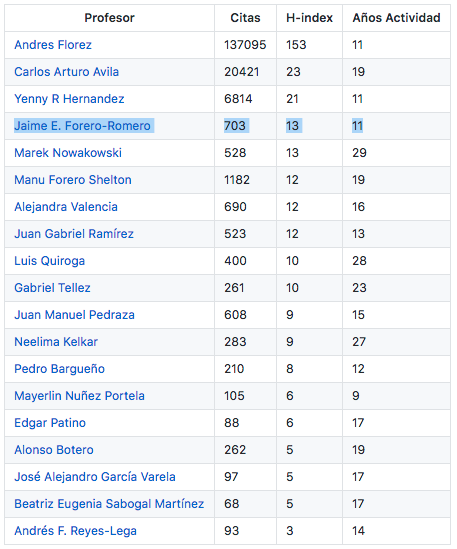
\includegraphics[scale=0.50]{scholar_fisica.png}
\caption{Figura para el problema 1. \url{https://github.com/forero/gsc/blob/master/info/fisica_uniandes.md}\label{table:fisica}}
\end{center}
\end{figure}


\begin{figure}[!h]
\begin{center}
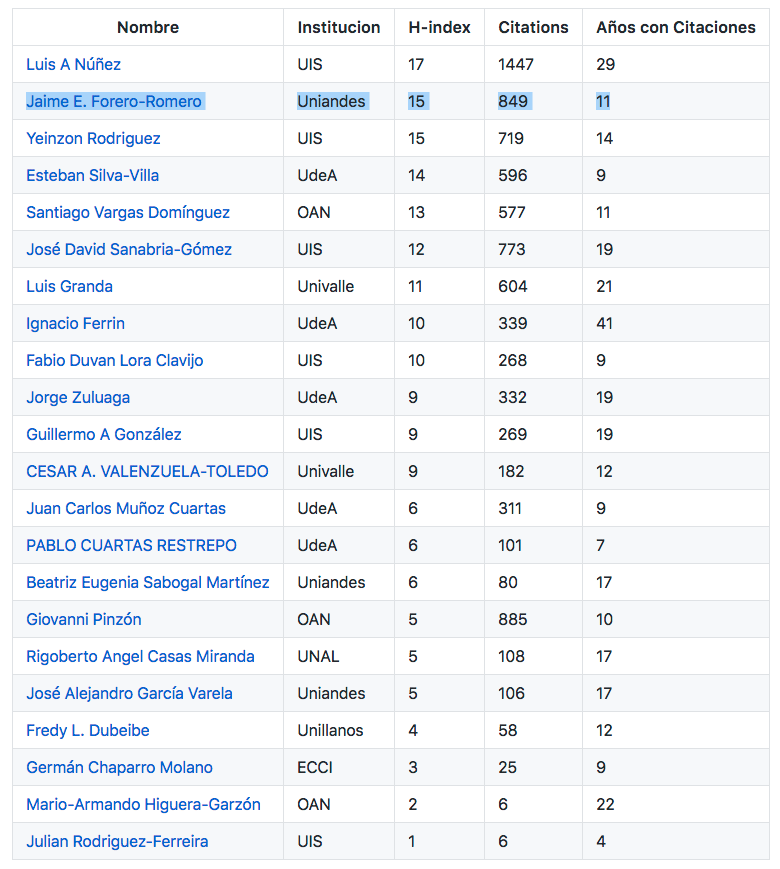
\includegraphics[scale=0.60]{scholar_astronomia.png}
\caption{Figura para el problema 1. \url{https://github.com/forero/gsc/blob/master/info/fisica_uniandes.md}\label{table:astro}}
\end{center}
\end{figure}



\newpage
\section{Desarrollo Institucional}


\subsection{Comit\'es y Coordinaciones}
\begin{itemize}
\item {2015-10. Representante del Departamento de F\'isica en el comit\'e
  de c\'omputo de alto rendimiento de la facultad de ciencias.}
\item {Desde 2016-10. Coordinador de los cursos computacionales de la carrera de
  F\'isica: Herramientas Computacionales, M\'etodos Computacionales y
  M\'etodos Computacionales avanzados.} 
\end{itemize}


\subsection{Visibilidad nacional e internacional}
\begin{itemize}
\item {Organizador de la una escuela Andina de Cosmolog\'ia (1 mes de
  duraci\'on, 4 instructores internacionales, 20 estudiantes de la
  regi\'on andina), Junio2015.}
\item {Co-organizador del segundo workshop Astronom\'ia en los Andes
  (cerca de 100 asistentes), Julio 2015.}
\item {Co-editor de las memorias del segundo workshop Astronom\'ia en
  los Andes, Julio 2015.}
\item {Lidero la Oficina Regional de Astronom\'ia para el
  Desarrollo. Esta Oficina es una red colaboraci\'on entre Colombia,
  Venezuela, Ecuador, Per\'u y Chile con el patrocinio de la Uni\'on
  Astron\'omica Internacional. La creaci\'on de la red se formaliz\'o
  en Julio del 2015 en la Universidad de los Andes.}   
\end{itemize}

\subsection{Presentaciones p\'ublicas}

\begin{tabular}{p{2.0cm} p{1.5cm} p{1.5cm} p{5.0cm} p{5.0cm}}\hline
Date & Country & City& Venue& Title\\\hline
19-02-2016 & Colombia & Medell\'in & Planetario de Medell\'in & Tiempos Cosmol\'ogicos\\
18-02-2016 & Colombia & Medell\'in & OPUS - Oficina de Arquitectura & Tiempos Cosmol\'ogicos\\
8-10-2015  & Colombia & Bogot\'a & Universidad Santo Tom\'as & Vida Cosmol\'ogica \\
21-05-2015 & Colombia & Bogot\'a & Conversatorio Maloka & De d\'onde vengo yo. Luz, estrellas y galaxias.\\
11-03-2015 & Colombia & B/manga & Caf\'e Cient\'ifico & Cielos Fluidos y Astronom\'ia Perif\'erica. Dos proyectos de Arte y Astronom\'ia.\\\hline
\end{tabular}

\subsection{Aparici\'on en medios de comunicaci\'on}

\begin{itemize}
\item Noviembre 2018. Entrevista sobre el proyecto DESI publicada en El Tiempo:

 \url{http://www.eltiempo.com/vida/ciencia/atlas-3d-mas-completo-del-universp-155450}.
\end{itemize}


\end{document}
